\section{Vision Transformer}\label{sec:vision-transformer}
Vision Transformers (ViTs), as introduced by Dosovitskiy et al. in 2020~\cite{Dosovitskiy2020}, build on the work of Vaswani et al.~\cite{Vaswani2017}, adapting the transformer architecture for image classification. 
ViTs leverage the transformer's strengths in handling sequential data by splitting an image into a sequence of $16\times16$ pixel patches and processing them through the transformer architecture just like tokens as explained below.
\begin{figure}[h]
    \centering
    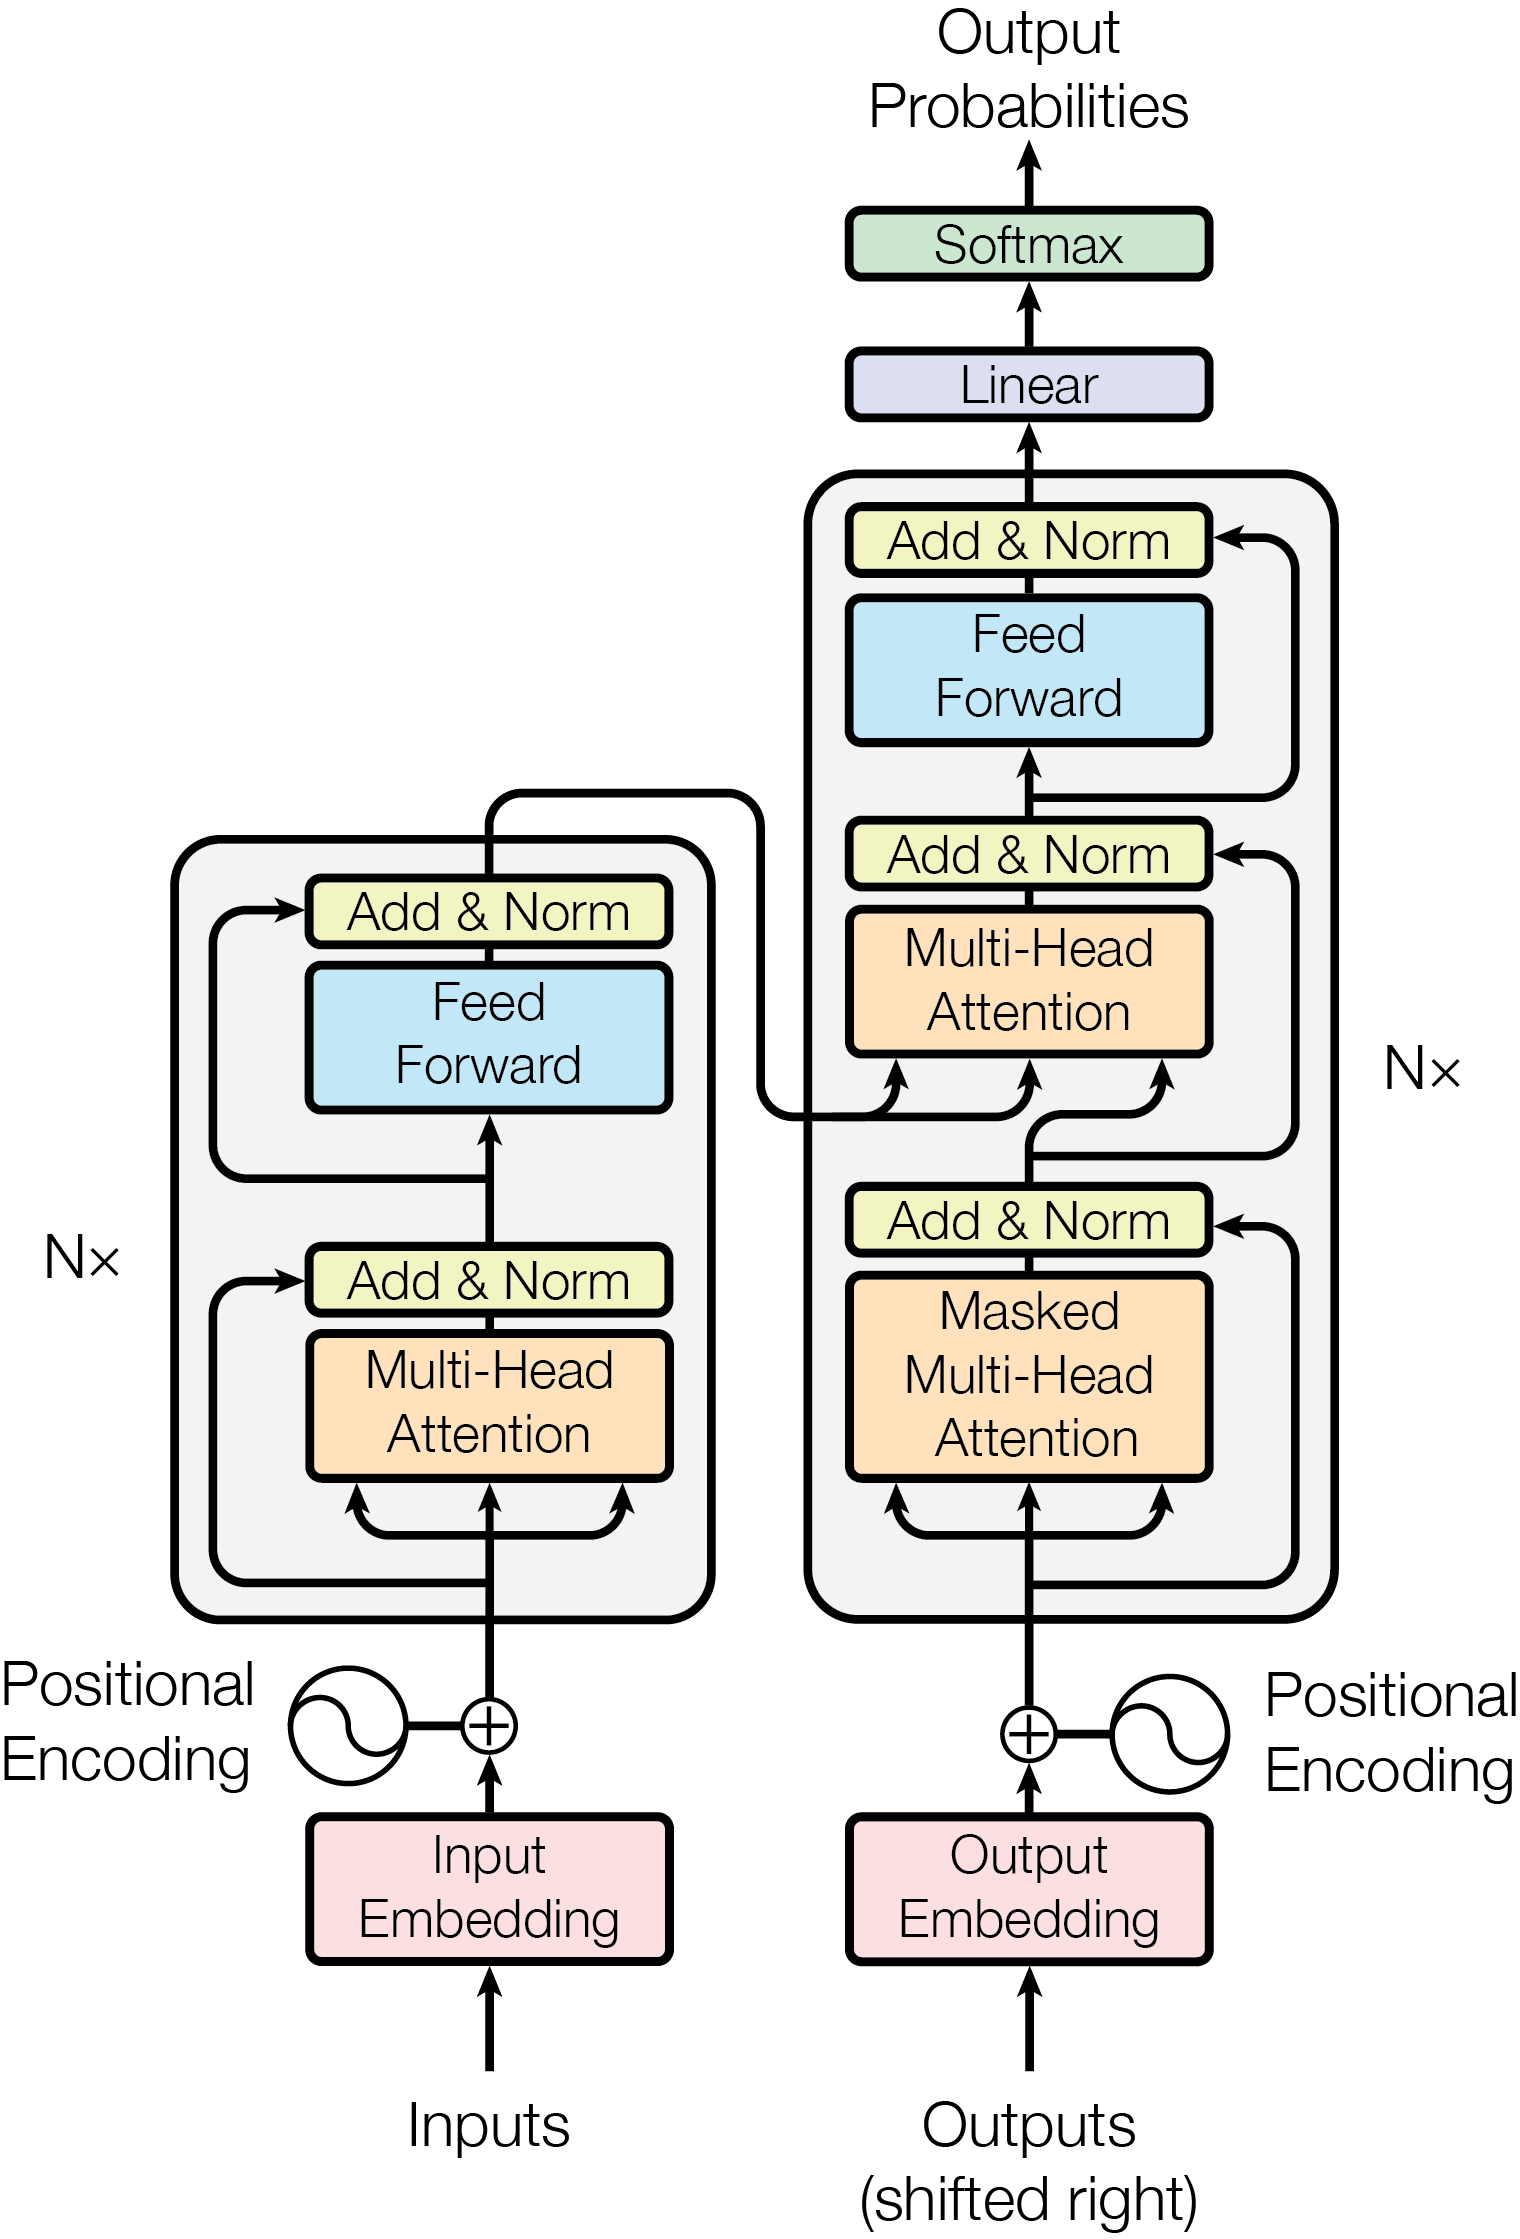
\includegraphics[width=0.3\textwidth]{images/TransformerArchitectureVaswani2017TransformerPage3.png}
    \caption[The original transformer architecture]{The transformer architecture (image from~\cite{Vaswani2017})}\label{fig:transformer}
\end{figure}

The original transformer architecture, designed for machine translation, consists of an encoder-decoder structure that processes input sequences through \emph{embedding layers}, \emph{positional encoding}, \emph{attention mechanisms}, and \emph{multi-layer perceptrons}. 
The following describes these components in the context of the original transformer architecture which is illustrated in Figure~\ref{fig:transformer}.

\textbf{Embedding Layer:} To ingest a sequence into a transformer, it is first split into smaller pieces called tokens, which can be words, subwords, or characters, and are then mapped into continuous vector representations called \emph{token vectors}. 
These \emph{token vectors} form the \emph{Embedding Matrix}.

\textbf{Positional Encoding:} Following the embedding a \emph{positional encoding matrix} is added to the \emph{Embedding Matrix}, which gives the model a hint of the order of the tokens in the sequence. 
This is needed as Transformers do not have an inductive bias about token order, unlike predecessors like Recurrent Neural Networks (RNNs)~\cite{Salehinejad2018} or Long Short-Term Memory (LSTM) networks~\cite{Hochreiter1997}.

\textbf{Encoder:} Next, the \emph{Embedding Matrix} is processed by a \emph{Multi-Head Attention} consisting of $h$ \emph{Attention Heads}.
The original paper achieved good results with $h=8$.
An Attention head first runs the \emph{Embedding Matrix} through three learnable linear layers $W^Q, W^K \&\, W^V$ in parallel, producing three matrices: \emph{query matrix} $Q$, \emph{key matrix} $K$, and \emph{value matrix} $V$ each $\in \mathrm{R}^{d_{\text{model}\times d_k}}$ with $d_{\text{model}}$ being the length of a token vector (512 in the original paper) and $d_k = \frac{d_{\text{model}}}{h}$. 
These terms are analogous to database operations, where the query matrix is the search query, the key matrix is the database, and the value matrix is the data in the database. 
These terms try to convey the intuition behind the attention mechanism.
These matrices are processed by one or more \emph{Attention Heads} as shown in Equation~\ref{eq:attention} to calculate the attention score using the Scaled Dot-Product Attention method. 
First the query matrix $Q$ and the transposed key matrix $K$ is multiplied, devided by the square of the dimension of the matrices $d_k$ and then normalized using softmax to prevent exploding gradients.
This dot product is the \emph{Attention Matrix} of dimension $d_{\text{model}}\times d_{\text{model}}$ which contains the \emph{Attention Scores} which can be interpreted as probabilities of how much a certain token is correlated to another token \textbf{Explained in a good manner here~\cite{Han2023}}. 
This \emph{Attention Matrix} then multiplied with the value matrix $V$ resulting in the weighted value matrix.
Having $h$ attention heads leads to $h$ weighted value matrices which are concatenated and processed by a final linear layer $W^O \in \mathrm{R}^{hd_k \times d_{\text{model}}}$.
\begin{equation}
    \text{Attention}(Q, K, V) = \text{softmax}\left(\frac{QK^{T}}{\sqrt{d_{k}}}\right)V
    \label{eq:attention}
\end{equation}
Following the multi-headed attention mechanism, the resulting 

\textbf{Decoder:} The original Transformer architecture includes an encoder-decoder structure, where the encoder processes the input sequence and the decoder generates the output sequence token by token. While both encoder and decoder consist of the same building blocks, the decoder uses a masked multi-headed attention mechanism, zeroing out the lower left triangle of the attention matrix containing the attention scores to prevent the model from attending to future tokens. 
Following that a multi-head cross attention was applied connecting the output of the encoder with the decoder.
Since then works such as the BERT framework by Devlin et al.~\cite{Devlin2018} have shown that the decoder is not inherently needed for tasks like language translation, or text generation allowing for a simplified \emph{Encoder Transformer} architecture.

This methodology is largely copied by the ViT architecture, though slightly adapted as shown in Table~\ref{tab:transformer_vit_comparison}.

\begin{table}[h!]
    \centering
    \begin{tabular}{|p{3cm}|p{5.5cm}|p{5.5cm}|}
    \hline
    \textbf{Component} & \textbf{Transformers} & \textbf{Vision Transformers (ViTs)} \\ \hline
    Embedding & Devides input sequence (e.g., a sentence) into tokens (e.g., syllables) and converts them into continuous vector representations, forming the Embedding Matrix. & Devides the input image into non-overlapping patches of size $16 \times 16$. Each patch is flattened and used as an embedding vector. All embedding vectors together form the Embedding Matrix.\\ \hline
    Position Embedding & Uses fixed 1-d sinusoidal positional encodings to encode the position of each token in the sequence.& Uses learnable position embeddings to better capture the spatial relationships between image patches.\\ \hline
    Encoder & Consists of a stack of identical layers, each with a multi-head self-attention mechanism and a position-wise fully connected feed-forward network. & Same as in Transformers.\\ \hline
    Decoder & Consists of a stack of identical layers, each with a multi-head self-attention mechanism and an multi-head cross attention connecting the output of the encoder with the decoder. The cross attention is followed by a position-wise fully connected feed-forward network. & Not applicable, as ViTs only use an encoder.\\ \hline
    Attention Mechanism & Computes attention scores using query (Q), key (K), and value (V) matrices. Multi-head attention allows the model to attend to different parts of the input sequence simultaneously. &Same as Transformer.\\ \hline
    Class Token & Not applicable. & Introduces a special class token appended to the sequence of patch embeddings, used for classification tasks by aggregating information from all patches.\\ \hline
    \end{tabular}
    \caption{Comparison of Components in Transformers and Vision Transformers}\label{tab:transformer_vit_comparison}
\end{table}

Using this simplified Transformer architecture, as visualized in Figure~\ref{fig:vit}, ViTs have demonstrated superior performance over state-of-the-art convolutional neural networks (CNNs) in several image classification tasks~\cite{Mauricio2023}. 
Since the original ViT paper, many more use cases beyond image classification have emerged for Transformers in the computer vision field, including anomaly detection, object/instance detection and segmentation, image compression and upscaling, dense/depth estimation~\cite{Ranftl2021}, and video image generation~\cite{Jamil2023}. 
Despite requiring significantly more training data than previous state-of-the-art CNN architectures, ViTs effectively leverage the transformer architecture to surpass the previous state of the art, highlighting the importance of unsupervised pre-training on large datasets and the flexibility of transformers in processing different types of data beyond natural language.
\begin{figure}
    \centering
    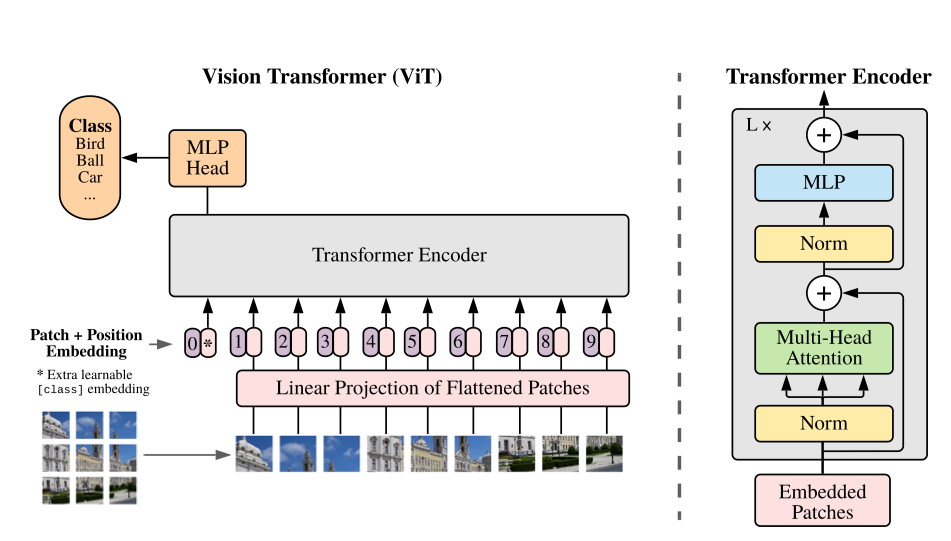
\includegraphics[width=0.8\textwidth]{images/vit_overview.png}
    \caption[The Vision Transformer architecture]{The Vision Transformer architecture (copied from~\cite{Dosovitskiy2020}).}\label{fig:vit}
\end{figure}

\section{Dino and DinoV2}
As mentioned in the privious Section~\ref{sec:vision-transformer}, ViTs are work very well for tasks like image classification and have shown superior performance over state-of-the-art convolutional neural networks (CNNs) in several image classification tasks.
So far ViTs were mostly trained in a supervised manner and needed a lot of labeled data to achieve state-of-the-art performance.
As labeled training data is expensive and time consuming to generate, it is very desirable to train models in an unsupervised manner.
Just a year after the introduction of the Vision Transformer, Caron et al.~\cite{Caron2021} introduced an approach to achieve exactly this called DINO (DIstilled NOt labeled), which is a framework for training in theory any network capable of ingesting image data using self-distillation without labels.
However the paper in particular emphasizes the synergy of Dino with Vision Transformers as a good compromise between performance and computational cost.
Dino is a usefull framework for tasks such as segmentation, depth estimation, and object detection, as it provides a good initialization for supervised fine-tuning.


As explained in~\cite{Phuong2019} destillation in machine learning is a method facilitating the transfer of knowledge from one model to another using a teacher-student model approach.
Often the teacher is a larger complex pretrained model which is used to train a much smaller stundent model. 
However, in the case of Dino the teacher is a non-pretrained model being trained in parallel with the student model. 
This process is called self-distillation, as no pretrained model is used to inject prexisting knowledge into the student model.

In a teacher stundent architecture the student tries to predict the output of the teacher model.
In Dino the students weights get updated using the classical gradient decend approach, while the teacher model is updated using a exponential moving average of the student model weights.
Caron et al. figured that in order to prevent a trivial solution where both teacher and student would start outputing the same output no regard to the input, it is enough to center the output of the teacher model to a mean of 0 and to apply a sharpened softmax function to the output by applying a temperatur parameter $\tau$ called temperatur to the softmax function as shown in equation~\ref{eq:sharp_softmax}. It makes very large values even larger and very small values even smaller.

\textbf{Architecture}

Dino is trained using a classical student teacher network approach, though the teacher is not a pretrained model but a model trained in parallel to the student model.
The Tracher model is largely the same as the student model, but the outputs follow a normalisation applying centering subtracting the mean and running the resulting outputs thorugh a shapened softmax function as shown in equation~\ref{eq:sharp_softmax}.

\begin{equation}
q_{i} = \frac{f_{i}}{|f_{i}|_{2}} \cdot \tau
\label{eq:sharp_softmax}
\end{equation}



- Attention Map right after training puts much attention on the main object of the image and less on the background. This already is a good start for segmentation
- Dino is trained unsupervised and places, when trained, images in to a latent vector, where similar images are close to each other, similar to how similar words are embedded close to each other when training a embedding on them. This could already be used for a k-nearest neighbor approach to classify images.
\subsection{Depth Estimation}
\subsection{Segmentation}

\section{Model Fine-Tuning}
Foundation Models (FMs), as defined in~\cite{Bommasani2021}, are models trained on a large variety of data using self-supervised learning sometimes even for weeks on hunderds of graphic processing units (GPUs) as e.g. the GPT3 model~\cite{Yuan2022} or the Florence CV Foundation Model by Yuan et al.~\cite{Yuan2021}.
These FMs can then fine-tuned doing few shot training, to tailor the FM to a specific task using several magnitutes less data as would be needed for training a model from scratch.
This saves a lot of computational cost and time as it often is enough to retrain only small parts of the FM, and most of the parameters/weights get frozen as well as that cost can be saved dataset which can be relativley small.
Mathematically, the straight forward way of fine-tuning a model is by retraining all parameters, which can be written as in equation~\ref{eq:finetuning} with $W_0$ being the pretrained weights and $\delta W$ the change in weights during fine-tuning.
\begin{equation}
    W' = W_0 + \delta W
    \label{eq:finetuning}
\end{equation}
This However still is relativley computationally intesive as the backpropagation has to be done for all parameters.
\textbf{DISCUSS IN GENERALL HOW PRETRAINING WORKS???}

A more efficient way of fine-tuning weight matrices is Low Rank Adaption (LoRA) as suggested by Hu et al.~\cite{Hu2021} in the context of transformer fine-tuning.
Hut et al. assume based on the the work of Aghajanyan et al.~\cite{Aghajanyan2020}, that the updated weight matrices $\delta W_n$ inside the attention heads of the transformer have a rank much lower then their dimensionality.
In order to utilize this assumption to more efficiently fine-tune a transformer the updated weight matrices $\delta W_n$ are decomposed into two matrices $A \in \mathbb{R}^{d \times r}$ and $B \in \mathbb{R}^{r \times k}$ with $r << d$ and $r << k$ as shown in equation~\ref{eq:lora}.
Hu et al. set the goal to use a maximum of 18M parameters for fine tuning the 173B parameter GPT3 model and created a grid search for optimizing the rank $r$ and which weight matrices to update.
Eventually they figured for their usecase a rank $r = 4$ and only applying updates to all key matrices $K$ and value matrices $V$ in the attention heads of the transformer performed the best.
Besides the advantage of significantly lowering the computational cost of only optimizing the $A$ and $B$ matrices, fine-tuning using LoRa does not increase inference times as the decomposed matrices are recomposed and added onto the original weight matrices $W_0$ after the fine tuning and therefor do not add any additional computation to the forward pass of the model.
\begin{equation}
    W = W_0 + BA
    \label{eq:lora}
\end{equation}

\begin{figure}
    \centering
    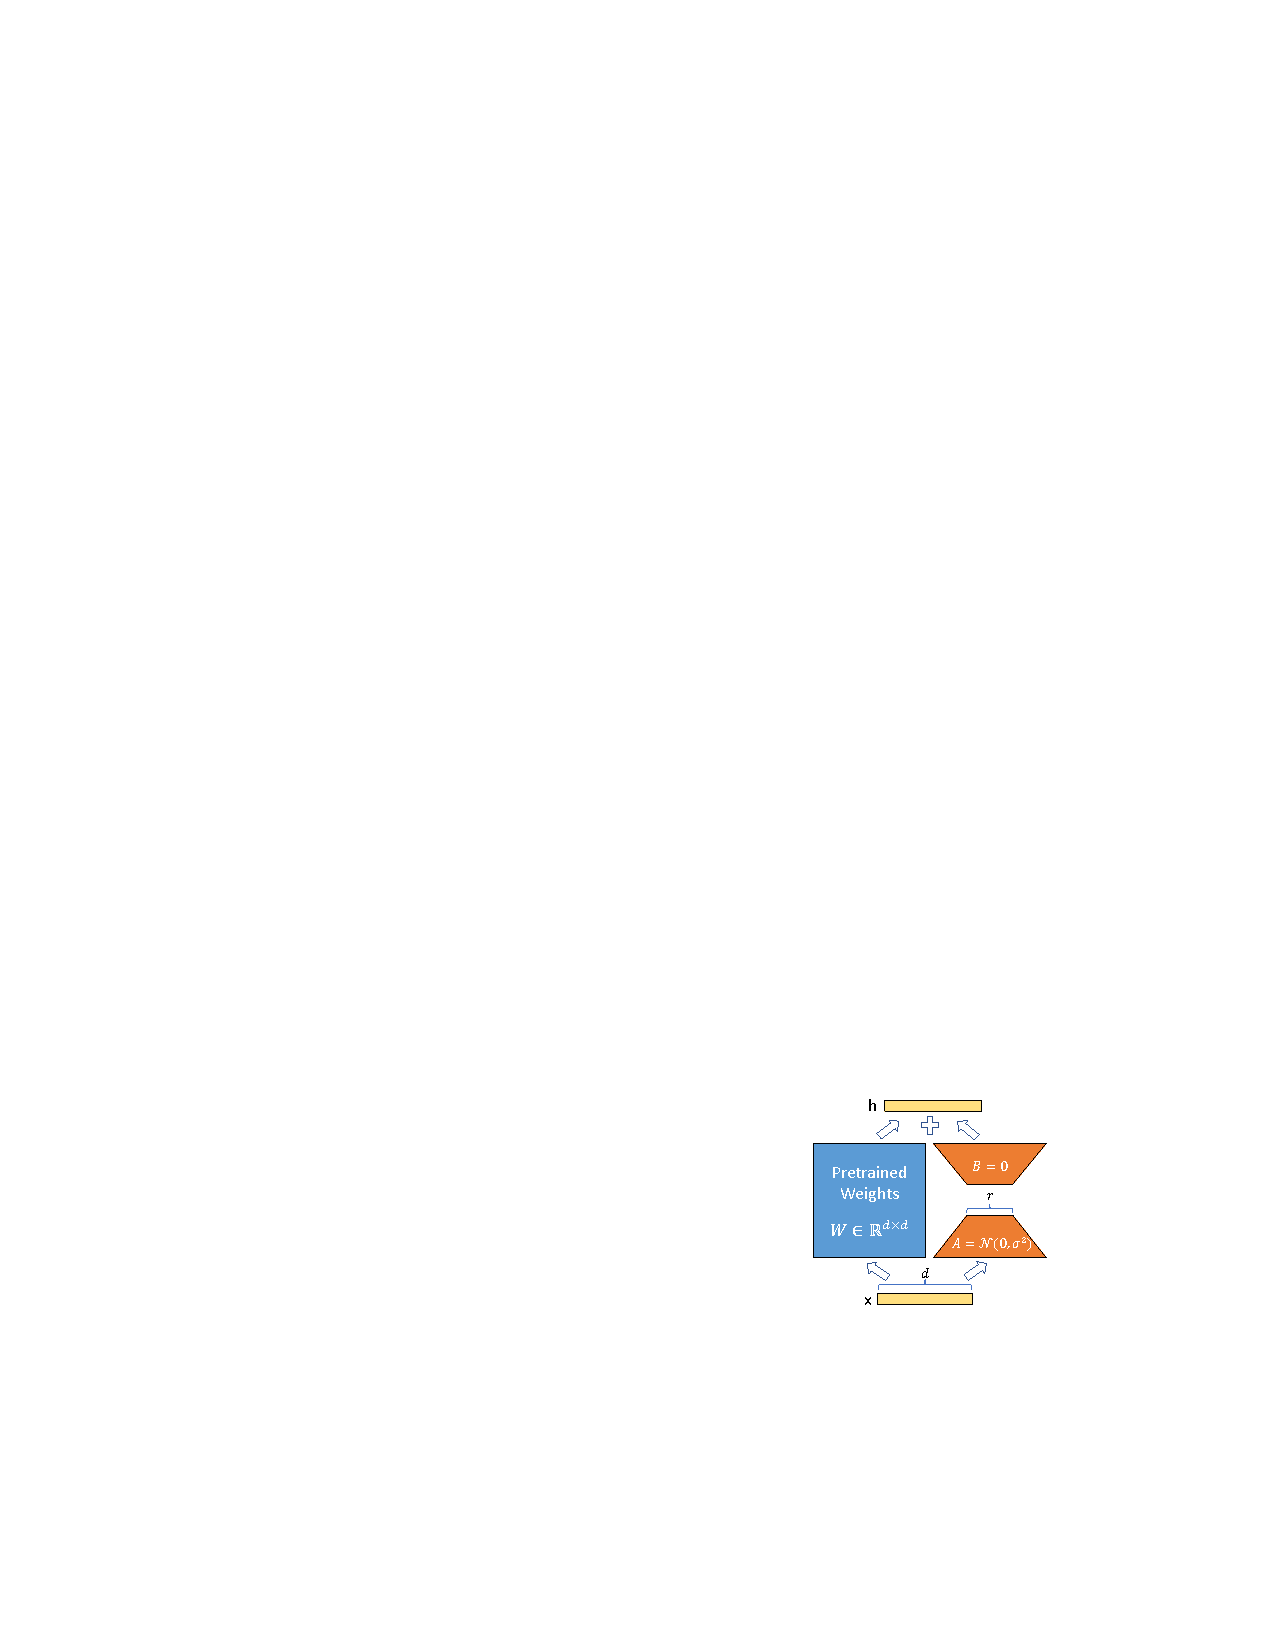
\includegraphics[width=0.5\textwidth]{images/Hu2021_LoraArch.pdf}
    \caption{LoRa architecture with the docomposed $\delta W_n = AB$ and their initialization  method (graphic lifted from~\cite{Hu2021})}\label{fig:loraarch}
\end{figure}

Another methodology of finetuning Neural Networks (NN) is to 